\documentclass[1p]{elsarticle_modified}
%\bibliographystyle{elsarticle-num}

%\usepackage[colorlinks]{hyperref}
%\usepackage{abbrmath_seonhwa} %\Abb, \Ascr, \Acal ,\Abf, \Afrak
\usepackage{amsfonts}
\usepackage{amssymb}
\usepackage{amsmath}
\usepackage{amsthm}
\usepackage{scalefnt}
\usepackage{amsbsy}
\usepackage{kotex}
\usepackage{caption}
\usepackage{subfig}
\usepackage{color}
\usepackage{graphicx}
\usepackage{xcolor} %% white, black, red, green, blue, cyan, magenta, yellow
\usepackage{float}
\usepackage{setspace}
\usepackage{hyperref}

\usepackage{tikz}
\usetikzlibrary{arrows}

\usepackage{multirow}
\usepackage{array} % fixed length table
\usepackage{hhline}

%%%%%%%%%%%%%%%%%%%%%
\makeatletter
\renewcommand*\env@matrix[1][\arraystretch]{%
	\edef\arraystretch{#1}%
	\hskip -\arraycolsep
	\let\@ifnextchar\new@ifnextchar
	\array{*\c@MaxMatrixCols c}}
\makeatother %https://tex.stackexchange.com/questions/14071/how-can-i-increase-the-line-spacing-in-a-matrix
%%%%%%%%%%%%%%%

\usepackage[normalem]{ulem}

\newcommand{\msout}[1]{\ifmmode\text{\sout{\ensuremath{#1}}}\else\sout{#1}\fi}
%SOURCE: \msout is \stkout macro in https://tex.stackexchange.com/questions/20609/strikeout-in-math-mode

\newcommand{\cancel}[1]{
	\ifmmode
	{\color{red}\msout{#1}}
	\else
	{\color{red}\sout{#1}}
	\fi
}

\newcommand{\add}[1]{
	{\color{blue}\uwave{#1}}
}

\newcommand{\replace}[2]{
	\ifmmode
	{\color{red}\msout{#1}}{\color{blue}\uwave{#2}}
	\else
	{\color{red}\sout{#1}}{\color{blue}\uwave{#2}}
	\fi
}

\newcommand{\Sol}{\mathcal{S}} %segment
\newcommand{\D}{D} %diagram
\newcommand{\A}{\mathcal{A}} %arc


%%%%%%%%%%%%%%%%%%%%%%%%%%%%%5 test

\def\sl{\operatorname{\textup{SL}}(2,\Cbb)}
\def\psl{\operatorname{\textup{PSL}}(2,\Cbb)}
\def\quan{\mkern 1mu \triangleright \mkern 1mu}

\theoremstyle{definition}
\newtheorem{thm}{Theorem}[section]
\newtheorem{prop}[thm]{Proposition}
\newtheorem{lem}[thm]{Lemma}
\newtheorem{ques}[thm]{Question}
\newtheorem{cor}[thm]{Corollary}
\newtheorem{defn}[thm]{Definition}
\newtheorem{exam}[thm]{Example}
\newtheorem{rmk}[thm]{Remark}
\newtheorem{alg}[thm]{Algorithm}

\newcommand{\I}{\sqrt{-1}}
\begin{document}

%\begin{frontmatter}
%
%\title{Boundary parabolic representations of knots up to 8 crossings}
%
%%% Group authors per affiliation:
%\author{Yunhi Cho} 
%\address{Department of Mathematics, University of Seoul, Seoul, Korea}
%\ead{yhcho@uos.ac.kr}
%
%
%\author{Seonhwa Kim} %\fnref{s_kim}}
%\address{Center for Geometry and Physics, Institute for Basic Science, Pohang, 37673, Korea}
%\ead{ryeona17@ibs.re.kr}
%
%\author{Hyuk Kim}
%\address{Department of Mathematical Sciences, Seoul National University, Seoul 08826, Korea}
%\ead{hyukkim@snu.ac.kr}
%
%\author{Seokbeom Yoon}
%\address{Department of Mathematical Sciences, Seoul National University, Seoul, 08826,  Korea}
%\ead{sbyoon15@snu.ac.kr}
%
%\begin{abstract}
%We find all boundary parabolic representation of knots up to 8 crossings.
%
%\end{abstract}
%\begin{keyword}
%    \MSC[2010] 57M25 
%\end{keyword}
%
%\end{frontmatter}

%\linenumbers
%\tableofcontents
%
\newcommand\colored[1]{\textcolor{white}{\rule[-0.35ex]{0.8em}{1.4ex}}\kern-0.8em\color{red} #1}%
%\newcommand\colored[1]{\textcolor{white}{ #1}\kern-2.17ex	\textcolor{white}{ #1}\kern-1.81ex	\textcolor{white}{ #1}\kern-2.15ex\color{red}#1	}

{\Large $\underline{12a_{1213}~(K12a_{1213})}$}

\setlength{\tabcolsep}{10pt}
\renewcommand{\arraystretch}{1.6}
\vspace{1cm}\begin{tabular}{m{100pt}>{\centering\arraybackslash}m{274pt}}
\multirow{5}{120pt}{
	\centering
	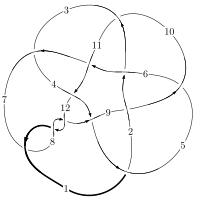
\includegraphics[width=112pt]{../../../GIT/diagram.site/Diagrams/png/2014_12a_1213.png}\\
\ \ \ A knot diagram\footnotemark}&
\allowdisplaybreaks
\textbf{Linearized knot diagam} \\
\cline{2-2}
 &
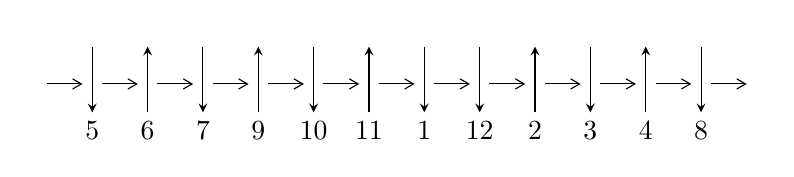
\begin{tikzpicture}[x=20pt, y=17pt]
	% nodes
	\node (C0) at (0, 0) {};
	\node (C1) at (1, 0) {};
	\node (C1U) at (1, +1) {};
	\node (C1D) at (1, -1) {5};

	\node (C2) at (2, 0) {};
	\node (C2U) at (2, +1) {};
	\node (C2D) at (2, -1) {6};

	\node (C3) at (3, 0) {};
	\node (C3U) at (3, +1) {};
	\node (C3D) at (3, -1) {7};

	\node (C4) at (4, 0) {};
	\node (C4U) at (4, +1) {};
	\node (C4D) at (4, -1) {9};

	\node (C5) at (5, 0) {};
	\node (C5U) at (5, +1) {};
	\node (C5D) at (5, -1) {10};

	\node (C6) at (6, 0) {};
	\node (C6U) at (6, +1) {};
	\node (C6D) at (6, -1) {11};

	\node (C7) at (7, 0) {};
	\node (C7U) at (7, +1) {};
	\node (C7D) at (7, -1) {1};

	\node (C8) at (8, 0) {};
	\node (C8U) at (8, +1) {};
	\node (C8D) at (8, -1) {12};

	\node (C9) at (9, 0) {};
	\node (C9U) at (9, +1) {};
	\node (C9D) at (9, -1) {2};

	\node (C10) at (10, 0) {};
	\node (C10U) at (10, +1) {};
	\node (C10D) at (10, -1) {3};

	\node (C11) at (11, 0) {};
	\node (C11U) at (11, +1) {};
	\node (C11D) at (11, -1) {4};

	\node (C12) at (12, 0) {};
	\node (C12U) at (12, +1) {};
	\node (C12D) at (12, -1) {8};
	\node (C13) at (13, 0) {};

	% arrows
	\draw[->,>={angle 60}]
	(C0) edge (C1) (C1) edge (C2) (C2) edge (C3) (C3) edge (C4) (C4) edge (C5) (C5) edge (C6) (C6) edge (C7) (C7) edge (C8) (C8) edge (C9) (C9) edge (C10) (C10) edge (C11) (C11) edge (C12) (C12) edge (C13) ;	\draw[->,>=stealth]
	(C1U) edge (C1D) (C2D) edge (C2U) (C3U) edge (C3D) (C4D) edge (C4U) (C5U) edge (C5D) (C6D) edge (C6U) (C7U) edge (C7D) (C8U) edge (C8D) (C9D) edge (C9U) (C10U) edge (C10D) (C11D) edge (C11U) (C12U) edge (C12D) ;
	\end{tikzpicture} \\
\hhline{~~} \\& 
\textbf{Solving Sequence} \\ \cline{2-2} 
 &
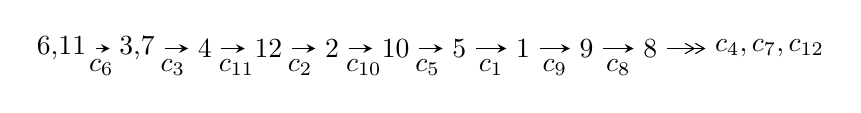
\begin{tikzpicture}[x=23pt, y=7pt]
	% node
	\node (A0) at (-1/8, 0) {6,11};
	\node (A1) at (17/16, 0) {3,7};
	\node (A2) at (17/8, 0) {4};
	\node (A3) at (25/8, 0) {12};
	\node (A4) at (33/8, 0) {2};
	\node (A5) at (41/8, 0) {10};
	\node (A6) at (49/8, 0) {5};
	\node (A7) at (57/8, 0) {1};
	\node (A8) at (65/8, 0) {9};
	\node (A9) at (73/8, 0) {8};
	\node (C1) at (1/2, -1) {$c_{6}$};
	\node (C2) at (13/8, -1) {$c_{3}$};
	\node (C3) at (21/8, -1) {$c_{11}$};
	\node (C4) at (29/8, -1) {$c_{2}$};
	\node (C5) at (37/8, -1) {$c_{10}$};
	\node (C6) at (45/8, -1) {$c_{5}$};
	\node (C7) at (53/8, -1) {$c_{1}$};
	\node (C8) at (61/8, -1) {$c_{9}$};
	\node (C9) at (69/8, -1) {$c_{8}$};
	\node (A10) at (11, 0) {$c_{4},c_{7},c_{12}$};

	% edge
	\draw[->,>=stealth]	
	(A0) edge (A1) (A1) edge (A2) (A2) edge (A3) (A3) edge (A4) (A4) edge (A5) (A5) edge (A6) (A6) edge (A7) (A7) edge (A8) (A8) edge (A9) ;
	\draw[->>,>={angle 60}]	
	(A9) edge (A10);
\end{tikzpicture} \\ 

\end{tabular} \\

\footnotetext{
The image of knot diagram is generated by the software ``\textbf{Draw programme}" developed by Andrew Bartholomew(\url{http://www.layer8.co.uk/maths/draw/index.htm\#Running-draw}), where we modified some parts for our purpose(\url{https://github.com/CATsTAILs/LinksPainter}).
}\phantom \\ \newline 
\centering \textbf{Ideals for irreducible components\footnotemark of $X_{\text{par}}$} 
 
\begin{align*}
I^u_{1}&=\langle 
-2.38072\times10^{36} u^{34}+2.10788\times10^{36} u^{33}+\cdots+2.31436\times10^{37} b-1.18052\times10^{37},\\
\phantom{I^u_{1}}&\phantom{= \langle  }1.34556\times10^{38} u^{34}+1.19595\times10^{38} u^{33}+\cdots+2.31436\times10^{37} a+9.18534\times10^{38},\;u^{35}+u^{34}+\cdots+8 u+1\rangle \\
I^u_{2}&=\langle 
-1.95779\times10^{17} u^{24}+2.57330\times10^{16} u^{23}+\cdots+3.09631\times10^{18} b+3.53328\times10^{18},\\
\phantom{I^u_{2}}&\phantom{= \langle  }-1.02595\times10^{18} u^{24}+1.39827\times10^{18} u^{23}+\cdots+1.23853\times10^{19} a+2.15965\times10^{19},\;u^{25}- u^{24}+\cdots-8 u-8\rangle \\
I^u_{3}&=\langle 
6.80801\times10^{870} u^{115}-1.02067\times10^{872} u^{114}+\cdots+2.89851\times10^{874} b+3.50026\times10^{875},\\
\phantom{I^u_{3}}&\phantom{= \langle  }-3.25101\times10^{874} u^{115}+2.16113\times10^{875} u^{114}+\cdots+1.53436\times10^{879} a+1.14628\times10^{881},\\
\phantom{I^u_{3}}&\phantom{= \langle  }u^{116}-15 u^{115}+\cdots-417760 u+52936\rangle \\
\\
\end{align*}
\raggedright * 3 irreducible components of $\dim_{\mathbb{C}}=0$, with total 176 representations.\\
\footnotetext{All coefficients of polynomials are rational numbers. But the coefficients are sometimes approximated in decimal forms when there is not enough margin.}
\newpage
\renewcommand{\arraystretch}{1}
\centering \section*{I. $I^u_{1}= \langle -2.38\times10^{36} u^{34}+2.11\times10^{36} u^{33}+\cdots+2.31\times10^{37} b-1.18\times10^{37},\;1.35\times10^{38} u^{34}+1.20\times10^{38} u^{33}+\cdots+2.31\times10^{37} a+9.19\times10^{38},\;u^{35}+u^{34}+\cdots+8 u+1 \rangle$}
\flushleft \textbf{(i) Arc colorings}\\
\begin{tabular}{m{7pt} m{180pt} m{7pt} m{180pt} }
\flushright $a_{6}=$&$\begin{pmatrix}1\\0\end{pmatrix}$ \\
\flushright $a_{11}=$&$\begin{pmatrix}0\\u\end{pmatrix}$ \\
\flushright $a_{3}=$&$\begin{pmatrix}-5.81398 u^{34}-5.16753 u^{33}+\cdots-72.6444 u-39.6884\\0.102867 u^{34}-0.0910783 u^{33}+\cdots-3.09658 u+0.510083\end{pmatrix}$ \\
\flushright $a_{7}=$&$\begin{pmatrix}1\\- u^2\end{pmatrix}$ \\
\flushright $a_{4}=$&$\begin{pmatrix}-5.70378 u^{34}-4.93508 u^{33}+\cdots-70.1903 u-39.5521\\0.182861 u^{34}+0.0177861 u^{33}+\cdots-2.00831 u+0.632342\end{pmatrix}$ \\
\flushright $a_{12}=$&$\begin{pmatrix}-33.5755 u^{34}-29.3518 u^{33}+\cdots-371.933 u-214.961\\0.712298 u^{34}+0.384179 u^{33}+\cdots+4.97991 u+5.59420\end{pmatrix}$ \\
\flushright $a_{2}=$&$\begin{pmatrix}-5.91684 u^{34}-5.07645 u^{33}+\cdots-69.5478 u-40.1985\\0.102867 u^{34}-0.0910783 u^{33}+\cdots-3.09658 u+0.510083\end{pmatrix}$ \\
\flushright $a_{10}=$&$\begin{pmatrix}-33.5988 u^{34}-29.1991 u^{33}+\cdots-363.943 u-212.176\\0.646444 u^{34}+0.433382 u^{33}+\cdots+6.82336 u+5.81398\end{pmatrix}$ \\
\flushright $a_{5}=$&$\begin{pmatrix}183.007 u^{34}+155.083 u^{33}+\cdots+1861.33 u+1147.00\\-4.39975 u^{34}-3.75957 u^{33}+\cdots-56.6144 u-33.5988\end{pmatrix}$ \\
\flushright $a_{1}=$&$\begin{pmatrix}24.6736 u^{34}+19.7265 u^{33}+\cdots+217.291 u+153.213\\-1.01831 u^{34}-1.24880 u^{33}+\cdots-18.6808 u-5.81082\end{pmatrix}$ \\
\flushright $a_{9}=$&$\begin{pmatrix}-34.4392 u^{34}-29.7788 u^{33}+\cdots-371.080 u-218.093\\0.840389 u^{34}+0.579717 u^{33}+\cdots+7.13622 u+5.91684\end{pmatrix}$ \\
\flushright $a_{8}=$&$\begin{pmatrix}-17.5414 u^{34}-15.2732 u^{33}+\cdots-157.692 u-91.1189\\-0.242519 u^{34}-0.107367 u^{33}+\cdots+8.50491 u+3.47843\end{pmatrix}$\\&\end{tabular}
\flushleft \textbf{(ii) Obstruction class $= -1$}\\~\\
\flushleft \textbf{(iii) Cusp Shapes $= -68.4106 u^{34}-55.3484 u^{33}+\cdots-679.743 u-457.303$}\\~\\
\newpage\renewcommand{\arraystretch}{1}
\flushleft \textbf{(iv) u-Polynomials at the component}\newline \\
\begin{tabular}{m{50pt}|m{274pt}}
Crossings & \hspace{64pt}u-Polynomials at each crossing \\
\hline $$\begin{aligned}c_{1},c_{3}\end{aligned}$$&$\begin{aligned}
&u^{35}-3 u^{34}+\cdots+13 u-1
\end{aligned}$\\
\hline $$\begin{aligned}c_{2}\end{aligned}$$&$\begin{aligned}
&u^{35}-25 u^{34}+\cdots+24576 u-2048
\end{aligned}$\\
\hline $$\begin{aligned}c_{4},c_{11}\end{aligned}$$&$\begin{aligned}
&u^{35}+7 u^{34}+\cdots-3 u+1
\end{aligned}$\\
\hline $$\begin{aligned}c_{5},c_{10}\end{aligned}$$&$\begin{aligned}
&u^{35}+5 u^{34}+\cdots-3 u+1
\end{aligned}$\\
\hline $$\begin{aligned}c_{6},c_{9}\end{aligned}$$&$\begin{aligned}
&u^{35}- u^{34}+\cdots+8 u-1
\end{aligned}$\\
\hline $$\begin{aligned}c_{7},c_{8},c_{12}\end{aligned}$$&$\begin{aligned}
&u^{35}+11 u^{34}+\cdots+384 u+32
\end{aligned}$\\
\hline
\end{tabular}\\~\\
\newpage\renewcommand{\arraystretch}{1}
\flushleft \textbf{(v) Riley Polynomials at the component}\newline \\
\begin{tabular}{m{50pt}|m{274pt}}
Crossings & \hspace{64pt}Riley Polynomials at each crossing \\
\hline $$\begin{aligned}c_{1},c_{3}\end{aligned}$$&$\begin{aligned}
&y^{35}+11 y^{34}+\cdots+29 y-1
\end{aligned}$\\
\hline $$\begin{aligned}c_{2}\end{aligned}$$&$\begin{aligned}
&y^{35}+15 y^{34}+\cdots-90177536 y-4194304
\end{aligned}$\\
\hline $$\begin{aligned}c_{4},c_{11}\end{aligned}$$&$\begin{aligned}
&y^{35}-51 y^{34}+\cdots+35 y-1
\end{aligned}$\\
\hline $$\begin{aligned}c_{5},c_{10}\end{aligned}$$&$\begin{aligned}
&y^{35}-39 y^{34}+\cdots+27 y-1
\end{aligned}$\\
\hline $$\begin{aligned}c_{6},c_{9}\end{aligned}$$&$\begin{aligned}
&y^{35}- y^{34}+\cdots+28 y-1
\end{aligned}$\\
\hline $$\begin{aligned}c_{7},c_{8},c_{12}\end{aligned}$$&$\begin{aligned}
&y^{35}+31 y^{34}+\cdots-7680 y-1024
\end{aligned}$\\
\hline
\end{tabular}\\~\\
\newpage\flushleft \textbf{(vi) Complex Volumes and Cusp Shapes}
$$\begin{array}{c|c|c}  
\text{Solutions to }I^u_{1}& \I (\text{vol} + \sqrt{-1}CS) & \text{Cusp shape}\\
 \hline 
\begin{aligned}
u &= -0.473191 + 0.955601 I \\
a &= \phantom{-}0.164857 - 0.773336 I \\
b &= \phantom{-}0.73632 - 1.23689 I\end{aligned}
 & -0.87815 - 2.10009 I & -6.29124 + 3.74115 I \\ \hline\begin{aligned}
u &= -0.473191 - 0.955601 I \\
a &= \phantom{-}0.164857 + 0.773336 I \\
b &= \phantom{-}0.73632 + 1.23689 I\end{aligned}
 & -0.87815 + 2.10009 I & -6.29124 - 3.74115 I \\ \hline\begin{aligned}
u &= -0.561860 + 0.934680 I \\
a &= \phantom{-}0.721974 + 0.705652 I \\
b &= \phantom{-}0.291621 + 0.692365 I\end{aligned}
 & \phantom{-}2.74039 + 5.52452 I & -2.61115 - 4.68081 I \\ \hline\begin{aligned}
u &= -0.561860 - 0.934680 I \\
a &= \phantom{-}0.721974 - 0.705652 I \\
b &= \phantom{-}0.291621 - 0.692365 I\end{aligned}
 & \phantom{-}2.74039 - 5.52452 I & -2.61115 + 4.68081 I \\ \hline\begin{aligned}
u &= \phantom{-}0.728850 + 0.833231 I \\
a &= \phantom{-}0.690527 - 0.506887 I \\
b &= \phantom{-}0.058923 - 0.690806 I\end{aligned}
 & -2.68642 - 1.48594 I & -5.76171 + 5.39125 I \\ \hline\begin{aligned}
u &= \phantom{-}0.728850 - 0.833231 I \\
a &= \phantom{-}0.690527 + 0.506887 I \\
b &= \phantom{-}0.058923 + 0.690806 I\end{aligned}
 & -2.68642 + 1.48594 I & -5.76171 - 5.39125 I \\ \hline\begin{aligned}
u &= \phantom{-}0.486606 + 1.044960 I \\
a &= \phantom{-}0.195291 - 0.498321 I \\
b &= \phantom{-}0.31826 - 1.73957 I\end{aligned}
 & -0.68127 + 1.41250 I & -3.06396 - 1.29126 I \\ \hline\begin{aligned}
u &= \phantom{-}0.486606 - 1.044960 I \\
a &= \phantom{-}0.195291 + 0.498321 I \\
b &= \phantom{-}0.31826 + 1.73957 I\end{aligned}
 & -0.68127 - 1.41250 I & -3.06396 + 1.29126 I \\ \hline\begin{aligned}
u &= -0.798627 + 0.123489 I \\
a &= -0.533379 - 0.839803 I \\
b &= \phantom{-}1.53890 - 0.84849 I\end{aligned}
 & \phantom{-}10.09970 - 2.57123 I & \phantom{-}7.26146 + 7.35567 I \\ \hline\begin{aligned}
u &= -0.798627 - 0.123489 I \\
a &= -0.533379 + 0.839803 I \\
b &= \phantom{-}1.53890 + 0.84849 I\end{aligned}
 & \phantom{-}10.09970 + 2.57123 I & \phantom{-}7.26146 - 7.35567 I\\
 \hline 
 \end{array}$$\newpage$$\begin{array}{c|c|c}  
\text{Solutions to }I^u_{1}& \I (\text{vol} + \sqrt{-1}CS) & \text{Cusp shape}\\
 \hline 
\begin{aligned}
u &= -0.300719 + 0.744013 I \\
a &= \phantom{-}0.189534 + 0.400172 I \\
b &= \phantom{-}0.03329 + 2.04106 I\end{aligned}
 & \phantom{-}7.92447 + 1.85760 I & -9.7550 - 10.3352 I \\ \hline\begin{aligned}
u &= -0.300719 - 0.744013 I \\
a &= \phantom{-}0.189534 - 0.400172 I \\
b &= \phantom{-}0.03329 - 2.04106 I\end{aligned}
 & \phantom{-}7.92447 - 1.85760 I & -9.7550 + 10.3352 I \\ \hline\begin{aligned}
u &= -0.663483 + 1.024170 I \\
a &= \phantom{-}0.189870 + 0.547409 I \\
b &= \phantom{-}0.43442 + 1.63061 I\end{aligned}
 & -1.65342 - 7.27417 I & -5.53901 + 7.92193 I \\ \hline\begin{aligned}
u &= -0.663483 - 1.024170 I \\
a &= \phantom{-}0.189870 - 0.547409 I \\
b &= \phantom{-}0.43442 - 1.63061 I\end{aligned}
 & -1.65342 + 7.27417 I & -5.53901 - 7.92193 I \\ \hline\begin{aligned}
u &= -1.023220 + 0.684265 I \\
a &= \phantom{-}0.615312 + 0.295804 I \\
b &= -0.320104 + 0.634624 I\end{aligned}
 & -0.17224 - 3.30186 I & \phantom{-}4.00752 - 4.42363 I \\ \hline\begin{aligned}
u &= -1.023220 - 0.684265 I \\
a &= \phantom{-}0.615312 - 0.295804 I \\
b &= -0.320104 - 0.634624 I\end{aligned}
 & -0.17224 + 3.30186 I & \phantom{-}4.00752 + 4.42363 I \\ \hline\begin{aligned}
u &= \phantom{-}0.748659 + 0.978142 I \\
a &= \phantom{-}0.165026 - 0.583693 I \\
b &= \phantom{-}0.55147 - 1.58642 I\end{aligned}
 & \phantom{-}4.79967 + 11.80520 I & -2.00000 - 8.67473 I \\ \hline\begin{aligned}
u &= \phantom{-}0.748659 - 0.978142 I \\
a &= \phantom{-}0.165026 + 0.583693 I \\
b &= \phantom{-}0.55147 + 1.58642 I\end{aligned}
 & \phantom{-}4.79967 - 11.80520 I & -2.00000 + 8.67473 I \\ \hline\begin{aligned}
u &= \phantom{-}0.894095 + 0.973220 I \\
a &= -0.088879 + 0.809478 I \\
b &= \phantom{-}1.13402 + 1.22065 I\end{aligned}
 & \phantom{-}0.21423 + 7.00365 I & \phantom{-0.000000 } 0. - 4.77334 I \\ \hline\begin{aligned}
u &= \phantom{-}0.894095 - 0.973220 I \\
a &= -0.088879 - 0.809478 I \\
b &= \phantom{-}1.13402 - 1.22065 I\end{aligned}
 & \phantom{-}0.21423 - 7.00365 I & \phantom{-0.000000 -}0. + 4.77334 I\\
 \hline 
 \end{array}$$\newpage$$\begin{array}{c|c|c}  
\text{Solutions to }I^u_{1}& \I (\text{vol} + \sqrt{-1}CS) & \text{Cusp shape}\\
 \hline 
\begin{aligned}
u &= \phantom{-}0.599988 + 0.271035 I \\
a &= -0.65464 + 1.47497 I \\
b &= \phantom{-}1.251390 + 0.566406 I\end{aligned}
 & \phantom{-}3.12898 + 2.04422 I & \phantom{-}4.59072 - 3.04484 I \\ \hline\begin{aligned}
u &= \phantom{-}0.599988 - 0.271035 I \\
a &= -0.65464 - 1.47497 I \\
b &= \phantom{-}1.251390 - 0.566406 I\end{aligned}
 & \phantom{-}3.12898 - 2.04422 I & \phantom{-}4.59072 + 3.04484 I \\ \hline\begin{aligned}
u &= -0.132382 + 0.519991 I \\
a &= \phantom{-}0.881561 - 0.313861 I \\
b &= -0.006740 - 0.358428 I\end{aligned}
 & -0.184960 - 1.127700 I & -2.22637 + 6.73061 I \\ \hline\begin{aligned}
u &= -0.132382 - 0.519991 I \\
a &= \phantom{-}0.881561 + 0.313861 I \\
b &= -0.006740 + 0.358428 I\end{aligned}
 & -0.184960 + 1.127700 I & -2.22637 - 6.73061 I \\ \hline\begin{aligned}
u &= -1.24107 + 0.80628 I \\
a &= -0.224566 - 0.903591 I \\
b &= \phantom{-}1.25904 - 1.04232 I\end{aligned}
 & \phantom{-}10.26990 - 7.64955 I & \phantom{-0.000000 } 0 \\ \hline\begin{aligned}
u &= -1.24107 - 0.80628 I \\
a &= -0.224566 + 0.903591 I \\
b &= \phantom{-}1.25904 + 1.04232 I\end{aligned}
 & \phantom{-}10.26990 + 7.64955 I & \phantom{-0.000000 } 0 \\ \hline\begin{aligned}
u &= \phantom{-}0.014885 + 0.497734 I \\
a &= \phantom{-}3.54266 - 2.08972 I \\
b &= \phantom{-}0.790590 - 0.123525 I\end{aligned}
 & \phantom{-}4.73898 + 2.59865 I & -10.3277 - 11.9450 I \\ \hline\begin{aligned}
u &= \phantom{-}0.014885 - 0.497734 I \\
a &= \phantom{-}3.54266 + 2.08972 I \\
b &= \phantom{-}0.790590 + 0.123525 I\end{aligned}
 & \phantom{-}4.73898 - 2.59865 I & -10.3277 + 11.9450 I \\ \hline\begin{aligned}
u &= \phantom{-}1.27290 + 0.91763 I \\
a &= -0.284094 + 0.896949 I \\
b &= \phantom{-}1.32093 + 1.01324 I\end{aligned}
 & \phantom{-}1.91254 + 10.46930 I & \phantom{-0.000000 } 0 \\ \hline\begin{aligned}
u &= \phantom{-}1.27290 - 0.91763 I \\
a &= -0.284094 - 0.896949 I \\
b &= \phantom{-}1.32093 - 1.01324 I\end{aligned}
 & \phantom{-}1.91254 - 10.46930 I & \phantom{-0.000000 } 0\\
 \hline 
 \end{array}$$\newpage$$\begin{array}{c|c|c}  
\text{Solutions to }I^u_{1}& \I (\text{vol} + \sqrt{-1}CS) & \text{Cusp shape}\\
 \hline 
\begin{aligned}
u &= -1.30681 + 0.93603 I \\
a &= -0.298108 - 0.936803 I \\
b &= \phantom{-}1.30845 - 0.96931 I\end{aligned}
 & \phantom{-}0.8251 - 15.9095 I & \phantom{-0.000000 } 0 \\ \hline\begin{aligned}
u &= -1.30681 - 0.93603 I \\
a &= -0.298108 + 0.936803 I \\
b &= \phantom{-}1.30845 + 0.96931 I\end{aligned}
 & \phantom{-}0.8251 + 15.9095 I & \phantom{-0.000000 } 0 \\ \hline\begin{aligned}
u &= \phantom{-}1.33364 + 0.94709 I \\
a &= -0.286932 + 0.961649 I \\
b &= \phantom{-}1.28491 + 0.95487 I\end{aligned}
 & \phantom{-}7.0349 + 20.2665 I & \phantom{-0.000000 } 0 \\ \hline\begin{aligned}
u &= \phantom{-}1.33364 - 0.94709 I \\
a &= -0.286932 - 0.961649 I \\
b &= \phantom{-}1.28491 - 0.95487 I\end{aligned}
 & \phantom{-}7.0349 - 20.2665 I & \phantom{-0.000000 } 0 \\ \hline\begin{aligned}
u &= -0.156518\phantom{ +0.000000I} \\
a &= -34.9720\phantom{ +0.000000I} \\
b &= \phantom{-}1.02859\phantom{ +0.000000I}\end{aligned}
 & \phantom{-}0.541372\phantom{ +0.000000I} & -424.140\phantom{ +0.000000I}\\
 \hline 
 \end{array}$$\newpage\newpage\renewcommand{\arraystretch}{1}
\centering \section*{II. $I^u_{2}= \langle -1.96\times10^{17} u^{24}+2.57\times10^{16} u^{23}+\cdots+3.10\times10^{18} b+3.53\times10^{18},\;-1.03\times10^{18} u^{24}+1.40\times10^{18} u^{23}+\cdots+1.24\times10^{19} a+2.16\times10^{19},\;u^{25}- u^{24}+\cdots-8 u-8 \rangle$}
\flushleft \textbf{(i) Arc colorings}\\
\begin{tabular}{m{7pt} m{180pt} m{7pt} m{180pt} }
\flushright $a_{6}=$&$\begin{pmatrix}1\\0\end{pmatrix}$ \\
\flushright $a_{11}=$&$\begin{pmatrix}0\\u\end{pmatrix}$ \\
\flushright $a_{3}=$&$\begin{pmatrix}0.0828360 u^{24}-0.112898 u^{23}+\cdots-1.89081 u-1.74372\\0.0632297 u^{24}-0.00831085 u^{23}+\cdots-1.12338 u-1.14113\end{pmatrix}$ \\
\flushright $a_{7}=$&$\begin{pmatrix}1\\- u^2\end{pmatrix}$ \\
\flushright $a_{4}=$&$\begin{pmatrix}0.0237886 u^{24}-0.0967624 u^{23}+\cdots-1.18962 u-0.362102\\0.0366311 u^{24}-0.0217545 u^{23}+\cdots-0.307708 u-0.797832\end{pmatrix}$ \\
\flushright $a_{12}=$&$\begin{pmatrix}0.0181137 u^{24}-0.00463381 u^{23}+\cdots-1.87039 u+0.341855\\0.0143600 u^{24}-0.0438065 u^{23}+\cdots+1.45977 u-0.114605\end{pmatrix}$ \\
\flushright $a_{2}=$&$\begin{pmatrix}0.0196063 u^{24}-0.104587 u^{23}+\cdots-0.767427 u-0.602598\\0.0632297 u^{24}-0.00831085 u^{23}+\cdots-1.12338 u-1.14113\end{pmatrix}$ \\
\flushright $a_{10}=$&$\begin{pmatrix}0.111772 u^{24}-0.130147 u^{23}+\cdots-0.329660 u-0.474602\\0.0300620 u^{24}-0.0258797 u^{23}+\cdots+1.08104 u-0.662688\end{pmatrix}$ \\
\flushright $a_{5}=$&$\begin{pmatrix}0.0470114 u^{24}-0.123522 u^{23}+\cdots-3.09053 u+0.235072\\0.0183753 u^{24}-0.0403395 u^{23}+\cdots-0.419572 u-0.894174\end{pmatrix}$ \\
\flushright $a_{1}=$&$\begin{pmatrix}0.0242955 u^{24}+0.00502972 u^{23}+\cdots+2.56668 u-1.33845\\0.0211853 u^{24}+0.0698665 u^{23}+\cdots-0.0456261 u+0.124634\end{pmatrix}$ \\
\flushright $a_{9}=$&$\begin{pmatrix}0.0267908 u^{24}-0.0521712 u^{23}+\cdots-0.775408 u-0.317751\\0.0849809 u^{24}-0.0779759 u^{23}+\cdots+0.445748 u-0.156850\end{pmatrix}$ \\
\flushright $a_{8}=$&$\begin{pmatrix}0.141789 u^{24}-0.189859 u^{23}+\cdots-1.17851 u-1.06959\\-0.0355395 u^{24}+0.0698178 u^{23}+\cdots+0.631153 u-0.896134\end{pmatrix}$\\&\end{tabular}
\flushleft \textbf{(ii) Obstruction class $= 1$}\\~\\
\flushleft \textbf{(iii) Cusp Shapes $= \frac{2452215208224550567}{12385251064844942024} u^{24}-\frac{846206872359813633}{12385251064844942024} u^{23}+\cdots-\frac{8471824635934717355}{3096312766211235506} u-\frac{6668781122666694554}{1548156383105617753}$}\\~\\
\newpage\renewcommand{\arraystretch}{1}
\flushleft \textbf{(iv) u-Polynomials at the component}\newline \\
\begin{tabular}{m{50pt}|m{274pt}}
Crossings & \hspace{64pt}u-Polynomials at each crossing \\
\hline $$\begin{aligned}c_{1},c_{3}\end{aligned}$$&$\begin{aligned}
&u^{25}-3 u^{24}+\cdots-40 u+56
\end{aligned}$\\
\hline $$\begin{aligned}c_{2}\end{aligned}$$&$\begin{aligned}
&u^{25}-8 u^{24}+\cdots-3 u-1
\end{aligned}$\\
\hline $$\begin{aligned}c_{4},c_{11}\end{aligned}$$&$\begin{aligned}
&8(8 u^{25}+8 u^{24}+\cdots+5 u^2+1)
\end{aligned}$\\
\hline $$\begin{aligned}c_{5},c_{10}\end{aligned}$$&$\begin{aligned}
&8(8 u^{25}-8 u^{24}+\cdots+11 u^2-1)
\end{aligned}$\\
\hline $$\begin{aligned}c_{6},c_{9}\end{aligned}$$&$\begin{aligned}
&u^{25}- u^{24}+\cdots-8 u-8
\end{aligned}$\\
\hline $$\begin{aligned}c_{7},c_{8}\end{aligned}$$&$\begin{aligned}
&u^{25}+2 u^{24}+\cdots-2 u+1
\end{aligned}$\\
\hline $$\begin{aligned}c_{12}\end{aligned}$$&$\begin{aligned}
&u^{25}-2 u^{24}+\cdots-2 u-1
\end{aligned}$\\
\hline
\end{tabular}\\~\\
\newpage\renewcommand{\arraystretch}{1}
\flushleft \textbf{(v) Riley Polynomials at the component}\newline \\
\begin{tabular}{m{50pt}|m{274pt}}
Crossings & \hspace{64pt}Riley Polynomials at each crossing \\
\hline $$\begin{aligned}c_{1},c_{3}\end{aligned}$$&$\begin{aligned}
&y^{25}-3 y^{24}+\cdots+19072 y-3136
\end{aligned}$\\
\hline $$\begin{aligned}c_{2}\end{aligned}$$&$\begin{aligned}
&y^{25}+10 y^{24}+\cdots+37 y-1
\end{aligned}$\\
\hline $$\begin{aligned}c_{4},c_{11}\end{aligned}$$&$\begin{aligned}
&64(64 y^{25}-448 y^{24}+\cdots-10 y-1)
\end{aligned}$\\
\hline $$\begin{aligned}c_{5},c_{10}\end{aligned}$$&$\begin{aligned}
&64(64 y^{25}-704 y^{24}+\cdots+22 y-1)
\end{aligned}$\\
\hline $$\begin{aligned}c_{6},c_{9}\end{aligned}$$&$\begin{aligned}
&y^{25}-7 y^{24}+\cdots+192 y-64
\end{aligned}$\\
\hline $$\begin{aligned}c_{7},c_{8},c_{12}\end{aligned}$$&$\begin{aligned}
&y^{25}+26 y^{24}+\cdots+46 y-1
\end{aligned}$\\
\hline
\end{tabular}\\~\\
\newpage\flushleft \textbf{(vi) Complex Volumes and Cusp Shapes}
$$\begin{array}{c|c|c}  
\text{Solutions to }I^u_{2}& \I (\text{vol} + \sqrt{-1}CS) & \text{Cusp shape}\\
 \hline 
\begin{aligned}
u &= \phantom{-}0.317550 + 0.877564 I \\
a &= -0.229611 + 0.699890 I \\
b &= -0.576807 + 1.289960 I\end{aligned}
 & -2.07306 + 0.81237 I & -8.44018 - 1.80632 I \\ \hline\begin{aligned}
u &= \phantom{-}0.317550 - 0.877564 I \\
a &= -0.229611 - 0.699890 I \\
b &= -0.576807 - 1.289960 I\end{aligned}
 & -2.07306 - 0.81237 I & -8.44018 + 1.80632 I \\ \hline\begin{aligned}
u &= \phantom{-}0.374639 + 0.814667 I \\
a &= -0.133763 - 0.490884 I \\
b &= -0.48326 - 1.89633 I\end{aligned}
 & \phantom{-}8.08619 - 1.60054 I & \phantom{-}4.91227 - 11.32939 I \\ \hline\begin{aligned}
u &= \phantom{-}0.374639 - 0.814667 I \\
a &= -0.133763 + 0.490884 I \\
b &= -0.48326 + 1.89633 I\end{aligned}
 & \phantom{-}8.08619 + 1.60054 I & \phantom{-}4.91227 + 11.32939 I \\ \hline\begin{aligned}
u &= -1.10397\phantom{ +0.000000I} \\
a &= -0.450023\phantom{ +0.000000I} \\
b &= \phantom{-}1.22211\phantom{ +0.000000I}\end{aligned}
 & \phantom{-}4.61475\phantom{ +0.000000I} & \phantom{-}8.27900\phantom{ +0.000000I} \\ \hline\begin{aligned}
u &= \phantom{-}1.081950 + 0.250410 I \\
a &= -0.465508 - 0.085599 I \\
b &= \phantom{-}1.077930 - 0.382096 I\end{aligned}
 & \phantom{-}9.67308 - 1.37757 I & \phantom{-}5.79906 + 0.19770 I \\ \hline\begin{aligned}
u &= \phantom{-}1.081950 - 0.250410 I \\
a &= -0.465508 + 0.085599 I \\
b &= \phantom{-}1.077930 + 0.382096 I\end{aligned}
 & \phantom{-}9.67308 + 1.37757 I & \phantom{-}5.79906 - 0.19770 I \\ \hline\begin{aligned}
u &= -1.010210 + 0.558270 I \\
a &= -0.685743 - 0.374548 I \\
b &= \phantom{-}0.123193 - 0.613480 I\end{aligned}
 & -0.50342 - 3.65382 I & -7.55217 + 7.75024 I \\ \hline\begin{aligned}
u &= -1.010210 - 0.558270 I \\
a &= -0.685743 + 0.374548 I \\
b &= \phantom{-}0.123193 + 0.613480 I\end{aligned}
 & -0.50342 + 3.65382 I & -7.55217 - 7.75024 I \\ \hline\begin{aligned}
u &= -0.888892 + 0.794377 I \\
a &= \phantom{-}0.20872 + 1.44121 I \\
b &= -1.098420 + 0.679608 I\end{aligned}
 & \phantom{-}1.26033 - 8.21911 I & \phantom{-}0.36152 + 8.38035 I\\
 \hline 
 \end{array}$$\newpage$$\begin{array}{c|c|c}  
\text{Solutions to }I^u_{2}& \I (\text{vol} + \sqrt{-1}CS) & \text{Cusp shape}\\
 \hline 
\begin{aligned}
u &= -0.888892 - 0.794377 I \\
a &= \phantom{-}0.20872 - 1.44121 I \\
b &= -1.098420 - 0.679608 I\end{aligned}
 & \phantom{-}1.26033 + 8.21911 I & \phantom{-}0.36152 - 8.38035 I \\ \hline\begin{aligned}
u &= -0.550547 + 1.107680 I \\
a &= -0.133124 + 0.611398 I \\
b &= -0.65999 + 1.56156 I\end{aligned}
 & \phantom{-}0.01650 - 2.22543 I & \phantom{-}4.06322 + 5.84619 I \\ \hline\begin{aligned}
u &= -0.550547 - 1.107680 I \\
a &= -0.133124 - 0.611398 I \\
b &= -0.65999 - 1.56156 I\end{aligned}
 & \phantom{-}0.01650 + 2.22543 I & \phantom{-}4.06322 - 5.84619 I \\ \hline\begin{aligned}
u &= -0.768453 + 0.973451 I \\
a &= -0.374681 + 0.879750 I \\
b &= -0.590219 + 0.962163 I\end{aligned}
 & \phantom{-}6.96474 - 11.65060 I & \phantom{-}2.09612 + 9.34091 I \\ \hline\begin{aligned}
u &= -0.768453 - 0.973451 I \\
a &= -0.374681 - 0.879750 I \\
b &= -0.590219 - 0.962163 I\end{aligned}
 & \phantom{-}6.96474 + 11.65060 I & \phantom{-}2.09612 - 9.34091 I \\ \hline\begin{aligned}
u &= \phantom{-}0.770593 + 1.061120 I \\
a &= -0.135159 - 0.791525 I \\
b &= -0.79038 - 1.22759 I\end{aligned}
 & \phantom{-}0.04224 + 8.07532 I & -0.32524 - 11.69521 I \\ \hline\begin{aligned}
u &= \phantom{-}0.770593 - 1.061120 I \\
a &= -0.135159 + 0.791525 I \\
b &= -0.79038 + 1.22759 I\end{aligned}
 & \phantom{-}0.04224 - 8.07532 I & -0.32524 + 11.69521 I \\ \hline\begin{aligned}
u &= \phantom{-}0.671501\phantom{ +0.000000I} \\
a &= -1.58450\phantom{ +0.000000I} \\
b &= -0.368886\phantom{ +0.000000I}\end{aligned}
 & -3.74850\phantom{ +0.000000I} & -10.8400\phantom{ +0.000000I} \\ \hline\begin{aligned}
u &= \phantom{-}0.942808 + 0.936636 I \\
a &= \phantom{-}0.128385 - 1.073180 I \\
b &= -1.10990 - 0.91866 I\end{aligned}
 & -0.63864 + 8.33929 I & -1.35664 - 7.88306 I \\ \hline\begin{aligned}
u &= \phantom{-}0.942808 - 0.936636 I \\
a &= \phantom{-}0.128385 + 1.073180 I \\
b &= -1.10990 + 0.91866 I\end{aligned}
 & -0.63864 - 8.33929 I & -1.35664 + 7.88306 I\\
 \hline 
 \end{array}$$\newpage$$\begin{array}{c|c|c}  
\text{Solutions to }I^u_{2}& \I (\text{vol} + \sqrt{-1}CS) & \text{Cusp shape}\\
 \hline 
\begin{aligned}
u &= -0.370104 + 0.321579 I \\
a &= -1.00930 - 1.83683 I \\
b &= -0.770228 - 0.418162 I\end{aligned}
 & -0.07970 - 3.22269 I & -5.25315 + 3.28753 I \\ \hline\begin{aligned}
u &= -0.370104 - 0.321579 I \\
a &= -1.00930 + 1.83683 I \\
b &= -0.770228 + 0.418162 I\end{aligned}
 & -0.07970 + 3.22269 I & -5.25315 - 3.28753 I \\ \hline\begin{aligned}
u &= -1.52760\phantom{ +0.000000I} \\
a &= -0.771960\phantom{ +0.000000I} \\
b &= \phantom{-}0.295403\phantom{ +0.000000I}\end{aligned}
 & \phantom{-}0.0461358\phantom{ +0.000000I} & -0.00449090\phantom{ +0.000000I} \\ \hline\begin{aligned}
u &= \phantom{-}1.58070 + 0.12470 I \\
a &= -0.766976 - 0.004982 I \\
b &= \phantom{-}0.303767 - 0.008468 I\end{aligned}
 & \phantom{-}4.75943 - 0.77091 I & -0.021983 + 0.140884 I \\ \hline\begin{aligned}
u &= \phantom{-}1.58070 - 0.12470 I \\
a &= -0.766976 + 0.004982 I \\
b &= \phantom{-}0.303767 + 0.008468 I\end{aligned}
 & \phantom{-}4.75943 + 0.77091 I & -0.021983 - 0.140884 I\\
 \hline 
 \end{array}$$\newpage\newpage\renewcommand{\arraystretch}{1}
\centering \section*{III. $I^u_{3}= \langle 6.81\times10^{870} u^{115}-1.02\times10^{872} u^{114}+\cdots+2.90\times10^{874} b+3.50\times10^{875},\;-3.25\times10^{874} u^{115}+2.16\times10^{875} u^{114}+\cdots+1.53\times10^{879} a+1.15\times10^{881},\;u^{116}-15 u^{115}+\cdots-417760 u+52936 \rangle$}
\flushleft \textbf{(i) Arc colorings}\\
\begin{tabular}{m{7pt} m{180pt} m{7pt} m{180pt} }
\flushright $a_{6}=$&$\begin{pmatrix}1\\0\end{pmatrix}$ \\
\flushright $a_{11}=$&$\begin{pmatrix}0\\u\end{pmatrix}$ \\
\flushright $a_{3}=$&$\begin{pmatrix}0.0000211881 u^{115}-0.000140850 u^{114}+\cdots+332.880 u-74.7079\\-0.000234880 u^{115}+0.00352137 u^{114}+\cdots+149.396 u-12.0761\end{pmatrix}$ \\
\flushright $a_{7}=$&$\begin{pmatrix}1\\- u^2\end{pmatrix}$ \\
\flushright $a_{4}=$&$\begin{pmatrix}0.000235461 u^{115}-0.00342005 u^{114}+\cdots+110.674 u-53.2636\\-0.000258566 u^{115}+0.00389995 u^{114}+\cdots+187.940 u-15.5229\end{pmatrix}$ \\
\flushright $a_{12}=$&$\begin{pmatrix}3.09589\times10^{-6} u^{115}-0.000142993 u^{114}+\cdots-40.8529 u-28.0315\\0.000275424 u^{115}-0.00411469 u^{114}+\cdots-170.695 u+9.50168\end{pmatrix}$ \\
\flushright $a_{2}=$&$\begin{pmatrix}0.000256068 u^{115}-0.00366222 u^{114}+\cdots+183.484 u-62.6318\\-0.000234880 u^{115}+0.00352137 u^{114}+\cdots+149.396 u-12.0761\end{pmatrix}$ \\
\flushright $a_{10}=$&$\begin{pmatrix}0.0000533118 u^{115}-0.00108371 u^{114}+\cdots-344.514 u-5.40386\\-0.0000839813 u^{115}+0.00125485 u^{114}+\cdots+31.0149 u-7.02085\end{pmatrix}$ \\
\flushright $a_{5}=$&$\begin{pmatrix}0.000186726 u^{115}-0.00263160 u^{114}+\cdots+357.144 u-102.550\\0.000175190 u^{115}-0.00262080 u^{114}+\cdots-52.7290 u+4.48737\end{pmatrix}$ \\
\flushright $a_{1}=$&$\begin{pmatrix}0.0000329485 u^{115}-0.000439958 u^{114}+\cdots+99.4761 u-74.2454\\-0.000110444 u^{115}+0.00159254 u^{114}+\cdots+30.4766 u-5.18938\end{pmatrix}$ \\
\flushright $a_{9}=$&$\begin{pmatrix}8.31143\times10^{-6} u^{115}+0.0000178873 u^{114}+\cdots+299.956 u-42.3593\\0.0000764582 u^{115}-0.00146462 u^{114}+\cdots-559.459 u+59.6749\end{pmatrix}$ \\
\flushright $a_{8}=$&$\begin{pmatrix}-0.000299255 u^{115}+0.00442911 u^{114}+\cdots-138.230 u+81.9995\\5.30386\times10^{-6} u^{115}-0.000162142 u^{114}+\cdots-178.360 u+16.8795\end{pmatrix}$\\&\end{tabular}
\flushleft \textbf{(ii) Obstruction class $= -1$}\\~\\
\flushleft \textbf{(iii) Cusp Shapes $= -0.00136918 u^{115}+0.0205831 u^{114}+\cdots+475.643 u-0.629277$}\\~\\
\newpage\renewcommand{\arraystretch}{1}
\flushleft \textbf{(iv) u-Polynomials at the component}\newline \\
\begin{tabular}{m{50pt}|m{274pt}}
Crossings & \hspace{64pt}u-Polynomials at each crossing \\
\hline $$\begin{aligned}c_{1},c_{3}\end{aligned}$$&$\begin{aligned}
&u^{116}+5 u^{115}+\cdots-293824 u-18872
\end{aligned}$\\
\hline $$\begin{aligned}c_{2}\end{aligned}$$&$\begin{aligned}
&(u^{58}+14 u^{57}+\cdots+2 u+1)^{2}
\end{aligned}$\\
\hline $$\begin{aligned}c_{4},c_{11}\end{aligned}$$&$\begin{aligned}
&8(8 u^{116}+104 u^{115}+\cdots-1.07834\times10^{8} u+3.68679\times10^{7})
\end{aligned}$\\
\hline $$\begin{aligned}c_{5},c_{10}\end{aligned}$$&$\begin{aligned}
&8(8 u^{116}+104 u^{115}+\cdots+65126 u-4735)
\end{aligned}$\\
\hline $$\begin{aligned}c_{6},c_{9}\end{aligned}$$&$\begin{aligned}
&u^{116}+15 u^{115}+\cdots+417760 u+52936
\end{aligned}$\\
\hline $$\begin{aligned}c_{7},c_{8},c_{12}\end{aligned}$$&$\begin{aligned}
&(u^{58}-6 u^{57}+\cdots-24 u+1)^{2}
\end{aligned}$\\
\hline
\end{tabular}\\~\\
\newpage\renewcommand{\arraystretch}{1}
\flushleft \textbf{(v) Riley Polynomials at the component}\newline \\
\begin{tabular}{m{50pt}|m{274pt}}
Crossings & \hspace{64pt}Riley Polynomials at each crossing \\
\hline $$\begin{aligned}c_{1},c_{3}\end{aligned}$$&$\begin{aligned}
&y^{116}-93 y^{115}+\cdots-74449976896 y+356152384
\end{aligned}$\\
\hline $$\begin{aligned}c_{2}\end{aligned}$$&$\begin{aligned}
&(y^{58}-14 y^{57}+\cdots-132 y+1)^{2}
\end{aligned}$\\
\hline $$\begin{aligned}c_{4},c_{11}\end{aligned}$$&$\begin{aligned}
&64(64 y^{116}-6720 y^{115}+\cdots-1.67721\times10^{17} y+1.35924\times10^{15})
\end{aligned}$\\
\hline $$\begin{aligned}c_{5},c_{10}\end{aligned}$$&$\begin{aligned}
&64(64 y^{116}-5184 y^{115}+\cdots-3.55007\times10^{9} y+2.24202\times10^{7})
\end{aligned}$\\
\hline $$\begin{aligned}c_{6},c_{9}\end{aligned}$$&$\begin{aligned}
&y^{116}-105 y^{115}+\cdots-367121525120 y+2802220096
\end{aligned}$\\
\hline $$\begin{aligned}c_{7},c_{8},c_{12}\end{aligned}$$&$\begin{aligned}
&(y^{58}+58 y^{57}+\cdots-272 y+1)^{2}
\end{aligned}$\\
\hline
\end{tabular}\\~\\
\newpage\flushleft \textbf{(vi) Complex Volumes and Cusp Shapes}
$$\begin{array}{c|c|c}  
\text{Solutions to }I^u_{3}& \I (\text{vol} + \sqrt{-1}CS) & \text{Cusp shape}\\
 \hline 
\begin{aligned}
u &= -1.01158\phantom{ +0.000000I} \\
a &= -8.79748\phantom{ +0.000000I} \\
b &= \phantom{-}0.0996704\phantom{ +0.000000I}\end{aligned}
 & \phantom{-}0.00210462\phantom{ +0.000000I} & \phantom{-0.000000 } 0 \\ \hline\begin{aligned}
u &= \phantom{-}0.979940 + 0.270868 I \\
a &= \phantom{-}1.27783 + 0.75838 I \\
b &= -0.673521 - 0.205430 I\end{aligned}
 & \phantom{-}10.39060 + 0.33751 I & \phantom{-0.000000 } 0 \\ \hline\begin{aligned}
u &= \phantom{-}0.979940 - 0.270868 I \\
a &= \phantom{-}1.27783 - 0.75838 I \\
b &= -0.673521 + 0.205430 I\end{aligned}
 & \phantom{-}10.39060 - 0.33751 I & \phantom{-0.000000 } 0 \\ \hline\begin{aligned}
u &= \phantom{-}0.260251 + 0.936468 I \\
a &= \phantom{-}0.995159 + 0.468241 I \\
b &= \phantom{-}0.540330 - 0.147934 I\end{aligned}
 & \phantom{-}0.160870 - 0.671910 I & \phantom{-0.000000 } 0 \\ \hline\begin{aligned}
u &= \phantom{-}0.260251 - 0.936468 I \\
a &= \phantom{-}0.995159 - 0.468241 I \\
b &= \phantom{-}0.540330 + 0.147934 I\end{aligned}
 & \phantom{-}0.160870 + 0.671910 I & \phantom{-0.000000 } 0 \\ \hline\begin{aligned}
u &= \phantom{-}0.899381 + 0.324843 I \\
a &= \phantom{-}0.02723 + 1.66548 I \\
b &= \phantom{-}0.327313 + 0.897043 I\end{aligned}
 & \phantom{-}6.88898 - 0.12974 I & \phantom{-0.000000 } 0 \\ \hline\begin{aligned}
u &= \phantom{-}0.899381 - 0.324843 I \\
a &= \phantom{-}0.02723 - 1.66548 I \\
b &= \phantom{-}0.327313 - 0.897043 I\end{aligned}
 & \phantom{-}6.88898 + 0.12974 I & \phantom{-0.000000 } 0 \\ \hline\begin{aligned}
u &= \phantom{-}0.500073 + 0.812320 I \\
a &= \phantom{-}1.002650 + 0.655796 I \\
b &= \phantom{-}0.677148 + 0.214687 I\end{aligned}
 & \phantom{-}4.86393 + 2.30422 I & \phantom{-0.000000 } 0 \\ \hline\begin{aligned}
u &= \phantom{-}0.500073 - 0.812320 I \\
a &= \phantom{-}1.002650 - 0.655796 I \\
b &= \phantom{-}0.677148 - 0.214687 I\end{aligned}
 & \phantom{-}4.86393 - 2.30422 I & \phantom{-0.000000 } 0 \\ \hline\begin{aligned}
u &= -0.692472 + 0.649475 I \\
a &= -0.818612 + 0.006859 I \\
b &= -0.767777 - 0.502166 I\end{aligned}
 & \phantom{-}1.15556 + 5.12365 I & \phantom{-0.000000 } 0\\
 \hline 
 \end{array}$$\newpage$$\begin{array}{c|c|c}  
\text{Solutions to }I^u_{3}& \I (\text{vol} + \sqrt{-1}CS) & \text{Cusp shape}\\
 \hline 
\begin{aligned}
u &= -0.692472 - 0.649475 I \\
a &= -0.818612 - 0.006859 I \\
b &= -0.767777 + 0.502166 I\end{aligned}
 & \phantom{-}1.15556 - 5.12365 I & \phantom{-0.000000 } 0 \\ \hline\begin{aligned}
u &= -0.941152 + 0.094794 I \\
a &= -0.138651 - 0.826278 I \\
b &= \phantom{-}1.013770 - 0.116777 I\end{aligned}
 & \phantom{-}3.73399 - 1.62934 I & \phantom{-0.000000 } 0 \\ \hline\begin{aligned}
u &= -0.941152 - 0.094794 I \\
a &= -0.138651 + 0.826278 I \\
b &= \phantom{-}1.013770 + 0.116777 I\end{aligned}
 & \phantom{-}3.73399 + 1.62934 I & \phantom{-0.000000 } 0 \\ \hline\begin{aligned}
u &= \phantom{-}0.234879 + 0.906360 I \\
a &= \phantom{-}0.130221 + 1.095070 I \\
b &= -0.751053 + 0.970955 I\end{aligned}
 & \phantom{-}1.50707 + 3.95116 I & \phantom{-0.000000 } 0 \\ \hline\begin{aligned}
u &= \phantom{-}0.234879 - 0.906360 I \\
a &= \phantom{-}0.130221 - 1.095070 I \\
b &= -0.751053 - 0.970955 I\end{aligned}
 & \phantom{-}1.50707 - 3.95116 I & \phantom{-0.000000 } 0 \\ \hline\begin{aligned}
u &= -0.817032 + 0.432974 I \\
a &= -0.409960 - 0.596017 I \\
b &= -0.751053 - 0.970955 I\end{aligned}
 & \phantom{-}1.50707 - 3.95116 I & \phantom{-0.000000 } 0 \\ \hline\begin{aligned}
u &= -0.817032 - 0.432974 I \\
a &= -0.409960 + 0.596017 I \\
b &= -0.751053 + 0.970955 I\end{aligned}
 & \phantom{-}1.50707 + 3.95116 I & \phantom{-0.000000 } 0 \\ \hline\begin{aligned}
u &= -0.905748 + 0.165780 I \\
a &= \phantom{-}0.90226 - 1.09537 I \\
b &= -0.704558 + 0.226547 I\end{aligned}
 & \phantom{-}3.59558 - 3.21071 I & \phantom{-0.000000 } 0 \\ \hline\begin{aligned}
u &= -0.905748 - 0.165780 I \\
a &= \phantom{-}0.90226 + 1.09537 I \\
b &= -0.704558 - 0.226547 I\end{aligned}
 & \phantom{-}3.59558 + 3.21071 I & \phantom{-0.000000 } 0 \\ \hline\begin{aligned}
u &= -0.873393 + 0.286666 I \\
a &= \phantom{-}0.212283 + 0.253939 I \\
b &= \phantom{-}1.53643 + 0.52266 I\end{aligned}
 & \phantom{-}7.01799 - 4.89766 I & \phantom{-0.000000 } 0\\
 \hline 
 \end{array}$$\newpage$$\begin{array}{c|c|c}  
\text{Solutions to }I^u_{3}& \I (\text{vol} + \sqrt{-1}CS) & \text{Cusp shape}\\
 \hline 
\begin{aligned}
u &= -0.873393 - 0.286666 I \\
a &= \phantom{-}0.212283 - 0.253939 I \\
b &= \phantom{-}1.53643 - 0.52266 I\end{aligned}
 & \phantom{-}7.01799 + 4.89766 I & \phantom{-0.000000 } 0 \\ \hline\begin{aligned}
u &= \phantom{-}0.713535 + 0.577768 I \\
a &= \phantom{-}0.63911 - 1.49896 I \\
b &= -0.664418 - 0.629619 I\end{aligned}
 & -3.06039 + 2.03547 I & \phantom{-0.000000 } 0 \\ \hline\begin{aligned}
u &= \phantom{-}0.713535 - 0.577768 I \\
a &= \phantom{-}0.63911 + 1.49896 I \\
b &= -0.664418 + 0.629619 I\end{aligned}
 & -3.06039 - 2.03547 I & \phantom{-0.000000 } 0 \\ \hline\begin{aligned}
u &= -0.763410 + 0.771723 I \\
a &= \phantom{-}0.028077 - 1.034150 I \\
b &= \phantom{-}0.559985 - 1.250220 I\end{aligned}
 & -0.90262 - 2.33430 I & \phantom{-0.000000 } 0 \\ \hline\begin{aligned}
u &= -0.763410 - 0.771723 I \\
a &= \phantom{-}0.028077 + 1.034150 I \\
b &= \phantom{-}0.559985 + 1.250220 I\end{aligned}
 & -0.90262 + 2.33430 I & \phantom{-0.000000 } 0 \\ \hline\begin{aligned}
u &= \phantom{-}1.078240 + 0.136226 I \\
a &= \phantom{-}2.71578 - 1.12355 I \\
b &= -0.366627 - 0.170388 I\end{aligned}
 & \phantom{-}5.01112 - 0.52164 I & \phantom{-0.000000 } 0 \\ \hline\begin{aligned}
u &= \phantom{-}1.078240 - 0.136226 I \\
a &= \phantom{-}2.71578 + 1.12355 I \\
b &= -0.366627 + 0.170388 I\end{aligned}
 & \phantom{-}5.01112 + 0.52164 I & \phantom{-0.000000 } 0 \\ \hline\begin{aligned}
u &= \phantom{-}0.493381 + 0.764958 I \\
a &= -0.15233 - 1.51824 I \\
b &= -1.115670 - 0.750715 I\end{aligned}
 & \phantom{-}1.01755 + 6.41344 I & \phantom{-0.000000 } 0 \\ \hline\begin{aligned}
u &= \phantom{-}0.493381 - 0.764958 I \\
a &= -0.15233 + 1.51824 I \\
b &= -1.115670 + 0.750715 I\end{aligned}
 & \phantom{-}1.01755 - 6.41344 I & \phantom{-0.000000 } 0 \\ \hline\begin{aligned}
u &= \phantom{-}0.637789 + 0.647820 I \\
a &= -0.356755 + 0.693103 I \\
b &= -0.713517 + 0.945516 I\end{aligned}
 & -3.36011 + 2.04094 I & \phantom{-0.000000 } 0\\
 \hline 
 \end{array}$$\newpage$$\begin{array}{c|c|c}  
\text{Solutions to }I^u_{3}& \I (\text{vol} + \sqrt{-1}CS) & \text{Cusp shape}\\
 \hline 
\begin{aligned}
u &= \phantom{-}0.637789 - 0.647820 I \\
a &= -0.356755 - 0.693103 I \\
b &= -0.713517 - 0.945516 I\end{aligned}
 & -3.36011 - 2.04094 I & \phantom{-0.000000 } 0 \\ \hline\begin{aligned}
u &= -0.898737 + 0.638239 I \\
a &= \phantom{-}0.62169 + 1.30815 I \\
b &= -0.767777 + 0.502166 I\end{aligned}
 & \phantom{-}1.15556 - 5.12365 I & \phantom{-0.000000 } 0 \\ \hline\begin{aligned}
u &= -0.898737 - 0.638239 I \\
a &= \phantom{-}0.62169 - 1.30815 I \\
b &= -0.767777 - 0.502166 I\end{aligned}
 & \phantom{-}1.15556 + 5.12365 I & \phantom{-0.000000 } 0 \\ \hline\begin{aligned}
u &= \phantom{-}1.135380 + 0.122044 I \\
a &= \phantom{-}0.086119 + 0.641099 I \\
b &= \phantom{-}1.026360 + 0.255290 I\end{aligned}
 & \phantom{-}9.75231 + 4.08244 I & \phantom{-0.000000 } 0 \\ \hline\begin{aligned}
u &= \phantom{-}1.135380 - 0.122044 I \\
a &= \phantom{-}0.086119 - 0.641099 I \\
b &= \phantom{-}1.026360 - 0.255290 I\end{aligned}
 & \phantom{-}9.75231 - 4.08244 I & \phantom{-0.000000 } 0 \\ \hline\begin{aligned}
u &= -0.746972 + 0.416669 I \\
a &= -1.49126 + 0.35281 I \\
b &= \phantom{-}1.026360 - 0.255290 I\end{aligned}
 & \phantom{-}9.75231 - 4.08244 I & \phantom{-0.000000 } 0 \\ \hline\begin{aligned}
u &= -0.746972 - 0.416669 I \\
a &= -1.49126 - 0.35281 I \\
b &= \phantom{-}1.026360 + 0.255290 I\end{aligned}
 & \phantom{-}9.75231 + 4.08244 I & \phantom{-0.000000 } 0 \\ \hline\begin{aligned}
u &= -0.843208 + 0.085931 I \\
a &= \phantom{-}0.57492 + 1.43425 I \\
b &= -1.15971 + 0.96631 I\end{aligned}
 & \phantom{-}9.5516 - 10.5652 I & \phantom{-0.000000 } 0 \\ \hline\begin{aligned}
u &= -0.843208 - 0.085931 I \\
a &= \phantom{-}0.57492 - 1.43425 I \\
b &= -1.15971 - 0.96631 I\end{aligned}
 & \phantom{-}9.5516 + 10.5652 I & \phantom{-0.000000 } 0 \\ \hline\begin{aligned}
u &= \phantom{-}0.823622 + 0.011430 I \\
a &= -0.53246 - 2.65982 I \\
b &= \phantom{-}0.432044 - 0.349969 I\end{aligned}
 & \phantom{-}4.00496 + 0.11590 I & \phantom{-0.000000 } 0\\
 \hline 
 \end{array}$$\newpage$$\begin{array}{c|c|c}  
\text{Solutions to }I^u_{3}& \I (\text{vol} + \sqrt{-1}CS) & \text{Cusp shape}\\
 \hline 
\begin{aligned}
u &= \phantom{-}0.823622 - 0.011430 I \\
a &= -0.53246 + 2.65982 I \\
b &= \phantom{-}0.432044 + 0.349969 I\end{aligned}
 & \phantom{-}4.00496 - 0.11590 I & \phantom{-0.000000 } 0 \\ \hline\begin{aligned}
u &= \phantom{-}0.788196 + 0.199185 I \\
a &= \phantom{-}1.06705 + 1.58260 I \\
b &= -0.733347 - 0.206691 I\end{aligned}
 & \phantom{-}3.00880 + 7.71935 I & \phantom{-0.000000 } 0 \\ \hline\begin{aligned}
u &= \phantom{-}0.788196 - 0.199185 I \\
a &= \phantom{-}1.06705 - 1.58260 I \\
b &= -0.733347 + 0.206691 I\end{aligned}
 & \phantom{-}3.00880 - 7.71935 I & \phantom{-0.000000 } 0 \\ \hline\begin{aligned}
u &= -0.709071 + 0.962261 I \\
a &= -0.310202 - 0.555623 I \\
b &= -0.690086 - 0.845429 I\end{aligned}
 & -0.358848 - 0.399308 I & \phantom{-0.000000 } 0 \\ \hline\begin{aligned}
u &= -0.709071 - 0.962261 I \\
a &= -0.310202 + 0.555623 I \\
b &= -0.690086 + 0.845429 I\end{aligned}
 & -0.358848 + 0.399308 I & \phantom{-0.000000 } 0 \\ \hline\begin{aligned}
u &= -0.751367 + 0.270441 I \\
a &= \phantom{-}1.42199 - 1.70934 I \\
b &= -0.736192 + 0.183930 I\end{aligned}
 & \phantom{-}9.1239 - 11.3929 I & \phantom{-0.000000 } 0 \\ \hline\begin{aligned}
u &= -0.751367 - 0.270441 I \\
a &= \phantom{-}1.42199 + 1.70934 I \\
b &= -0.736192 - 0.183930 I\end{aligned}
 & \phantom{-}9.1239 + 11.3929 I & \phantom{-0.000000 } 0 \\ \hline\begin{aligned}
u &= \phantom{-}0.759086 + 0.167333 I \\
a &= -1.038420 - 0.884858 I \\
b &= \phantom{-}1.013770 + 0.116777 I\end{aligned}
 & \phantom{-}3.73399 + 1.62934 I & \phantom{-0.000000 } 0. - 5.11449 I \\ \hline\begin{aligned}
u &= \phantom{-}0.759086 - 0.167333 I \\
a &= -1.038420 + 0.884858 I \\
b &= \phantom{-}1.013770 - 0.116777 I\end{aligned}
 & \phantom{-}3.73399 - 1.62934 I & \phantom{-0.000000 -}0. + 5.11449 I \\ \hline\begin{aligned}
u &= -0.153958 + 0.761524 I \\
a &= -0.055312 - 1.198320 I \\
b &= -0.713517 - 0.945516 I\end{aligned}
 & -3.36011 - 2.04094 I & -8.79412 + 5.85740 I\\
 \hline 
 \end{array}$$\newpage$$\begin{array}{c|c|c}  
\text{Solutions to }I^u_{3}& \I (\text{vol} + \sqrt{-1}CS) & \text{Cusp shape}\\
 \hline 
\begin{aligned}
u &= -0.153958 - 0.761524 I \\
a &= -0.055312 + 1.198320 I \\
b &= -0.713517 + 0.945516 I\end{aligned}
 & -3.36011 + 2.04094 I & -8.79412 - 5.85740 I \\ \hline\begin{aligned}
u &= \phantom{-}0.786939 + 0.941766 I \\
a &= -0.448228 + 0.268724 I \\
b &= -0.664418 + 0.629619 I\end{aligned}
 & -3.06039 - 2.03547 I & \phantom{-0.000000 } 0 \\ \hline\begin{aligned}
u &= \phantom{-}0.786939 - 0.941766 I \\
a &= -0.448228 - 0.268724 I \\
b &= -0.664418 - 0.629619 I\end{aligned}
 & -3.06039 + 2.03547 I & \phantom{-0.000000 } 0 \\ \hline\begin{aligned}
u &= \phantom{-}0.754748\phantom{ +0.000000I} \\
a &= \phantom{-}0.222173\phantom{ +0.000000I} \\
b &= \phantom{-}1.85662\phantom{ +0.000000I}\end{aligned}
 & \phantom{-}2.24749\phantom{ +0.000000I} & \phantom{-}9.28120\phantom{ +0.000000I} \\ \hline\begin{aligned}
u &= -0.757678 + 0.996838 I \\
a &= -0.016211 + 1.208650 I \\
b &= -1.088980 + 0.799671 I\end{aligned}
 & -2.18513 - 8.49069 I & \phantom{-0.000000 } 0 \\ \hline\begin{aligned}
u &= -0.757678 - 0.996838 I \\
a &= -0.016211 - 1.208650 I \\
b &= -1.088980 - 0.799671 I\end{aligned}
 & -2.18513 + 8.49069 I & \phantom{-0.000000 } 0 \\ \hline\begin{aligned}
u &= -0.256825 + 0.697678 I \\
a &= \phantom{-}0.20777 + 1.57054 I \\
b &= -0.690086 + 0.845429 I\end{aligned}
 & -0.358848 + 0.399308 I & -2.00000 + 0. I\phantom{ +0.000000I} \\ \hline\begin{aligned}
u &= -0.256825 - 0.697678 I \\
a &= \phantom{-}0.20777 - 1.57054 I \\
b &= -0.690086 - 0.845429 I\end{aligned}
 & -0.358848 - 0.399308 I & -2.00000 + 0. I\phantom{ +0.000000I} \\ \hline\begin{aligned}
u &= \phantom{-}1.022720 + 0.775036 I \\
a &= -0.242532 + 1.097970 I \\
b &= \phantom{-}0.677280 + 1.077370 I\end{aligned}
 & -1.81586 + 7.53048 I & \phantom{-0.000000 } 0 \\ \hline\begin{aligned}
u &= \phantom{-}1.022720 - 0.775036 I \\
a &= -0.242532 - 1.097970 I \\
b &= \phantom{-}0.677280 - 1.077370 I\end{aligned}
 & -1.81586 - 7.53048 I & \phantom{-0.000000 } 0\\
 \hline 
 \end{array}$$\newpage$$\begin{array}{c|c|c}  
\text{Solutions to }I^u_{3}& \I (\text{vol} + \sqrt{-1}CS) & \text{Cusp shape}\\
 \hline 
\begin{aligned}
u &= -1.098930 + 0.694343 I \\
a &= \phantom{-}0.325265 + 1.289590 I \\
b &= -1.076520 + 0.823273 I\end{aligned}
 & \phantom{-}2.54061 - 10.54650 I & \phantom{-0.000000 } 0 \\ \hline\begin{aligned}
u &= -1.098930 - 0.694343 I \\
a &= \phantom{-}0.325265 - 1.289590 I \\
b &= -1.076520 - 0.823273 I\end{aligned}
 & \phantom{-}2.54061 + 10.54650 I & \phantom{-0.000000 } 0 \\ \hline\begin{aligned}
u &= \phantom{-}1.054200 + 0.808278 I \\
a &= \phantom{-}0.283751 - 1.221210 I \\
b &= -1.088980 - 0.799671 I\end{aligned}
 & -2.18513 + 8.49069 I & \phantom{-0.000000 } 0 \\ \hline\begin{aligned}
u &= \phantom{-}1.054200 - 0.808278 I \\
a &= \phantom{-}0.283751 + 1.221210 I \\
b &= -1.088980 + 0.799671 I\end{aligned}
 & -2.18513 - 8.49069 I & \phantom{-0.000000 } 0 \\ \hline\begin{aligned}
u &= -1.115170 + 0.723638 I \\
a &= -0.339399 - 1.173380 I \\
b &= \phantom{-}0.681559 - 0.993043 I\end{aligned}
 & \phantom{-}4.42249 - 11.60810 I & \phantom{-0.000000 } 0 \\ \hline\begin{aligned}
u &= -1.115170 - 0.723638 I \\
a &= -0.339399 + 1.173380 I \\
b &= \phantom{-}0.681559 + 0.993043 I\end{aligned}
 & \phantom{-}4.42249 + 11.60810 I & \phantom{-0.000000 } 0 \\ \hline\begin{aligned}
u &= -0.578647 + 0.272996 I \\
a &= \phantom{-}0.57081 - 2.37898 I \\
b &= \phantom{-}0.540330 - 0.147934 I\end{aligned}
 & \phantom{-}0.160870 - 0.671910 I & -2.15622 + 10.18820 I \\ \hline\begin{aligned}
u &= -0.578647 - 0.272996 I \\
a &= \phantom{-}0.57081 + 2.37898 I \\
b &= \phantom{-}0.540330 + 0.147934 I\end{aligned}
 & \phantom{-}0.160870 + 0.671910 I & -2.15622 - 10.18820 I \\ \hline\begin{aligned}
u &= \phantom{-}0.625939 + 0.130720 I \\
a &= \phantom{-}0.69693 - 1.62006 I \\
b &= -1.27363 - 0.94541 I\end{aligned}
 & \phantom{-}2.36016 + 7.44357 I & \phantom{-}2.72331 - 8.71572 I \\ \hline\begin{aligned}
u &= \phantom{-}0.625939 - 0.130720 I \\
a &= \phantom{-}0.69693 + 1.62006 I \\
b &= -1.27363 + 0.94541 I\end{aligned}
 & \phantom{-}2.36016 - 7.44357 I & \phantom{-}2.72331 + 8.71572 I\\
 \hline 
 \end{array}$$\newpage$$\begin{array}{c|c|c}  
\text{Solutions to }I^u_{3}& \I (\text{vol} + \sqrt{-1}CS) & \text{Cusp shape}\\
 \hline 
\begin{aligned}
u &= -0.533442 + 1.266060 I \\
a &= -0.080396 - 0.396039 I \\
b &= -0.441070 - 0.879956 I\end{aligned}
 & -0.767799 - 0.707140 I & \phantom{-0.000000 } 0 \\ \hline\begin{aligned}
u &= -0.533442 - 1.266060 I \\
a &= -0.080396 + 0.396039 I \\
b &= -0.441070 + 0.879956 I\end{aligned}
 & -0.767799 + 0.707140 I & \phantom{-0.000000 } 0 \\ \hline\begin{aligned}
u &= \phantom{-}0.503153 + 0.320623 I \\
a &= \phantom{-}0.813514 + 1.061800 I \\
b &= -1.04228 + 1.32124 I\end{aligned}
 & \phantom{-}8.59840 + 2.41577 I & \phantom{-}10.35447 - 1.07003 I \\ \hline\begin{aligned}
u &= \phantom{-}0.503153 - 0.320623 I \\
a &= \phantom{-}0.813514 - 1.061800 I \\
b &= -1.04228 - 1.32124 I\end{aligned}
 & \phantom{-}8.59840 - 2.41577 I & \phantom{-}10.35447 + 1.07003 I \\ \hline\begin{aligned}
u &= -1.12741 + 0.87171 I \\
a &= \phantom{-}0.366742 + 1.095350 I \\
b &= -1.115670 + 0.750715 I\end{aligned}
 & \phantom{-}1.01755 - 6.41344 I & \phantom{-0.000000 } 0 \\ \hline\begin{aligned}
u &= -1.12741 - 0.87171 I \\
a &= \phantom{-}0.366742 - 1.095350 I \\
b &= -1.115670 - 0.750715 I\end{aligned}
 & \phantom{-}1.01755 + 6.41344 I & \phantom{-0.000000 } 0 \\ \hline\begin{aligned}
u &= \phantom{-}0.85018 + 1.18672 I \\
a &= -0.035511 - 1.062400 I \\
b &= -1.076520 - 0.823273 I\end{aligned}
 & \phantom{-}2.54061 + 10.54650 I & \phantom{-0.000000 } 0 \\ \hline\begin{aligned}
u &= \phantom{-}0.85018 - 1.18672 I \\
a &= -0.035511 + 1.062400 I \\
b &= -1.076520 + 0.823273 I\end{aligned}
 & \phantom{-}2.54061 - 10.54650 I & \phantom{-0.000000 } 0 \\ \hline\begin{aligned}
u &= -1.31779 + 0.75264 I \\
a &= \phantom{-}0.154248 + 0.681986 I \\
b &= -0.704558 + 0.226547 I\end{aligned}
 & \phantom{-}3.59558 - 3.21071 I & \phantom{-0.000000 } 0 \\ \hline\begin{aligned}
u &= -1.31779 - 0.75264 I \\
a &= \phantom{-}0.154248 - 0.681986 I \\
b &= -0.704558 - 0.226547 I\end{aligned}
 & \phantom{-}3.59558 + 3.21071 I & \phantom{-0.000000 } 0\\
 \hline 
 \end{array}$$\newpage$$\begin{array}{c|c|c}  
\text{Solutions to }I^u_{3}& \I (\text{vol} + \sqrt{-1}CS) & \text{Cusp shape}\\
 \hline 
\begin{aligned}
u &= \phantom{-}0.07393 + 1.52551 I \\
a &= \phantom{-}0.188483 - 0.440292 I \\
b &= \phantom{-}0.559985 - 1.250220 I\end{aligned}
 & -0.90262 - 2.33430 I & \phantom{-0.000000 } 0 \\ \hline\begin{aligned}
u &= \phantom{-}0.07393 - 1.52551 I \\
a &= \phantom{-}0.188483 + 0.440292 I \\
b &= \phantom{-}0.559985 + 1.250220 I\end{aligned}
 & -0.90262 + 2.33430 I & \phantom{-0.000000 } 0 \\ \hline\begin{aligned}
u &= \phantom{-}1.24493 + 0.88674 I \\
a &= \phantom{-}0.003312 - 0.789661 I \\
b &= -0.733347 - 0.206691 I\end{aligned}
 & \phantom{-}3.00880 + 7.71935 I & \phantom{-0.000000 } 0 \\ \hline\begin{aligned}
u &= \phantom{-}1.24493 - 0.88674 I \\
a &= \phantom{-}0.003312 + 0.789661 I \\
b &= -0.733347 + 0.206691 I\end{aligned}
 & \phantom{-}3.00880 - 7.71935 I & \phantom{-0.000000 } 0 \\ \hline\begin{aligned}
u &= -0.453705 + 0.067556 I \\
a &= \phantom{-}1.09810 - 1.34637 I \\
b &= -1.45141 - 1.20638 I\end{aligned}
 & \phantom{-}1.44591 + 2.04368 I & \phantom{-}6.19891 - 7.65821 I \\ \hline\begin{aligned}
u &= -0.453705 - 0.067556 I \\
a &= \phantom{-}1.09810 + 1.34637 I \\
b &= -1.45141 + 1.20638 I\end{aligned}
 & \phantom{-}1.44591 - 2.04368 I & \phantom{-}6.19891 + 7.65821 I \\ \hline\begin{aligned}
u &= -0.404516 + 0.160541 I \\
a &= \phantom{-}0.82003 + 2.15188 I \\
b &= -0.441070 + 0.879956 I\end{aligned}
 & -0.767799 + 0.707140 I & -1.24485 - 4.27067 I \\ \hline\begin{aligned}
u &= -0.404516 - 0.160541 I \\
a &= \phantom{-}0.82003 - 2.15188 I \\
b &= -0.441070 - 0.879956 I\end{aligned}
 & -0.767799 - 0.707140 I & -1.24485 + 4.27067 I \\ \hline\begin{aligned}
u &= -1.25351 + 0.99399 I \\
a &= -0.115660 + 0.761637 I \\
b &= -0.736192 + 0.183930 I\end{aligned}
 & \phantom{-}9.1239 - 11.3929 I & \phantom{-0.000000 } 0 \\ \hline\begin{aligned}
u &= -1.25351 - 0.99399 I \\
a &= -0.115660 - 0.761637 I \\
b &= -0.736192 - 0.183930 I\end{aligned}
 & \phantom{-}9.1239 + 11.3929 I & \phantom{-0.000000 } 0\\
 \hline 
 \end{array}$$\newpage$$\begin{array}{c|c|c}  
\text{Solutions to }I^u_{3}& \I (\text{vol} + \sqrt{-1}CS) & \text{Cusp shape}\\
 \hline 
\begin{aligned}
u &= -0.36377 + 1.56837 I \\
a &= \phantom{-}0.237958 + 0.409554 I \\
b &= \phantom{-}0.677280 + 1.077370 I\end{aligned}
 & -1.81586 + 7.53048 I & \phantom{-0.000000 } 0 \\ \hline\begin{aligned}
u &= -0.36377 - 1.56837 I \\
a &= \phantom{-}0.237958 - 0.409554 I \\
b &= \phantom{-}0.677280 - 1.077370 I\end{aligned}
 & -1.81586 - 7.53048 I & \phantom{-0.000000 } 0 \\ \hline\begin{aligned}
u &= \phantom{-}1.51405 + 0.60574 I \\
a &= -0.697006 + 0.215750 I \\
b &= \phantom{-}1.53643 + 0.52266 I\end{aligned}
 & \phantom{-}7.01799 - 4.89766 I & \phantom{-0.000000 } 0 \\ \hline\begin{aligned}
u &= \phantom{-}1.51405 - 0.60574 I \\
a &= -0.697006 - 0.215750 I \\
b &= \phantom{-}1.53643 - 0.52266 I\end{aligned}
 & \phantom{-}7.01799 + 4.89766 I & \phantom{-0.000000 } 0 \\ \hline\begin{aligned}
u &= -1.12746 + 1.17840 I \\
a &= \phantom{-}0.077668 + 0.451088 I \\
b &= -1.04228 + 1.32124 I\end{aligned}
 & \phantom{-}8.59840 + 2.41577 I & \phantom{-0.000000 } 0 \\ \hline\begin{aligned}
u &= -1.12746 - 1.17840 I \\
a &= \phantom{-}0.077668 - 0.451088 I \\
b &= -1.04228 - 1.32124 I\end{aligned}
 & \phantom{-}8.59840 - 2.41577 I & \phantom{-0.000000 } 0 \\ \hline\begin{aligned}
u &= \phantom{-}1.52190 + 0.73520 I \\
a &= \phantom{-}0.091226 - 0.489453 I \\
b &= -0.673521 - 0.205430 I\end{aligned}
 & \phantom{-}10.39060 + 0.33751 I & \phantom{-0.000000 } 0 \\ \hline\begin{aligned}
u &= \phantom{-}1.52190 - 0.73520 I \\
a &= \phantom{-}0.091226 + 0.489453 I \\
b &= -0.673521 + 0.205430 I\end{aligned}
 & \phantom{-}10.39060 - 0.33751 I & \phantom{-0.000000 } 0 \\ \hline\begin{aligned}
u &= -1.37300 + 1.05302 I \\
a &= \phantom{-}0.247643 + 0.695092 I \\
b &= -1.27363 + 0.94541 I\end{aligned}
 & \phantom{-}2.36016 - 7.44357 I & \phantom{-0.000000 } 0 \\ \hline\begin{aligned}
u &= -1.37300 - 1.05302 I \\
a &= \phantom{-}0.247643 - 0.695092 I \\
b &= -1.27363 - 0.94541 I\end{aligned}
 & \phantom{-}2.36016 + 7.44357 I & \phantom{-0.000000 } 0\\
 \hline 
 \end{array}$$\newpage$$\begin{array}{c|c|c}  
\text{Solutions to }I^u_{3}& \I (\text{vol} + \sqrt{-1}CS) & \text{Cusp shape}\\
 \hline 
\begin{aligned}
u &= \phantom{-}0.47056 + 1.67845 I \\
a &= \phantom{-}0.246842 - 0.393743 I \\
b &= \phantom{-}0.681559 - 0.993043 I\end{aligned}
 & \phantom{-}4.42249 - 11.60810 I & \phantom{-0.000000 } 0 \\ \hline\begin{aligned}
u &= \phantom{-}0.47056 - 1.67845 I \\
a &= \phantom{-}0.246842 + 0.393743 I \\
b &= \phantom{-}0.681559 + 0.993043 I\end{aligned}
 & \phantom{-}4.42249 + 11.60810 I & \phantom{-0.000000 } 0 \\ \hline\begin{aligned}
u &= \phantom{-}1.34694 + 1.13133 I \\
a &= \phantom{-}0.119382 - 0.726589 I \\
b &= -1.15971 - 0.96631 I\end{aligned}
 & \phantom{-}9.5516 + 10.5652 I & \phantom{-0.000000 } 0 \\ \hline\begin{aligned}
u &= \phantom{-}1.34694 - 1.13133 I \\
a &= \phantom{-}0.119382 + 0.726589 I \\
b &= -1.15971 + 0.96631 I\end{aligned}
 & \phantom{-}9.5516 - 10.5652 I & \phantom{-0.000000 } 0 \\ \hline\begin{aligned}
u &= -1.81161\phantom{ +0.000000I} \\
a &= -0.588467\phantom{ +0.000000I} \\
b &= \phantom{-}1.85662\phantom{ +0.000000I}\end{aligned}
 & \phantom{-}2.24749\phantom{ +0.000000I} & \phantom{-0.000000 } 0 \\ \hline\begin{aligned}
u &= \phantom{-}0.149531 + 0.022926 I \\
a &= \phantom{-}3.10840 + 10.08440 I \\
b &= \phantom{-}0.677148 + 0.214687 I\end{aligned}
 & \phantom{-}4.86393 + 2.30422 I & \phantom{-}5.13678 - 7.19189 I \\ \hline\begin{aligned}
u &= \phantom{-}0.149531 - 0.022926 I \\
a &= \phantom{-}3.10840 - 10.08440 I \\
b &= \phantom{-}0.677148 - 0.214687 I\end{aligned}
 & \phantom{-}4.86393 - 2.30422 I & \phantom{-}5.13678 + 7.19189 I \\ \hline\begin{aligned}
u &= -0.07748 + 1.89589 I \\
a &= \phantom{-}0.421157 + 0.046884 I \\
b &= \phantom{-}0.432044 + 0.349969 I\end{aligned}
 & \phantom{-}4.00496 - 0.11590 I & \phantom{-0.000000 } 0 \\ \hline\begin{aligned}
u &= -0.07748 - 1.89589 I \\
a &= \phantom{-}0.421157 - 0.046884 I \\
b &= \phantom{-}0.432044 - 0.349969 I\end{aligned}
 & \phantom{-}4.00496 + 0.11590 I & \phantom{-0.000000 } 0 \\ \hline\begin{aligned}
u &= \phantom{-}1.51690 + 1.21579 I \\
a &= \phantom{-}0.246784 - 0.484838 I \\
b &= -1.45141 - 1.20638 I\end{aligned}
 & \phantom{-}1.44591 + 2.04368 I & \phantom{-0.000000 } 0\\
 \hline 
 \end{array}$$\newpage$$\begin{array}{c|c|c}  
\text{Solutions to }I^u_{3}& \I (\text{vol} + \sqrt{-1}CS) & \text{Cusp shape}\\
 \hline 
\begin{aligned}
u &= \phantom{-}1.51690 - 1.21579 I \\
a &= \phantom{-}0.246784 + 0.484838 I \\
b &= -1.45141 + 1.20638 I\end{aligned}
 & \phantom{-}1.44591 - 2.04368 I & \phantom{-0.000000 } 0 \\ \hline\begin{aligned}
u &= \phantom{-}0.00499 + 1.94799 I \\
a &= \phantom{-}0.181253 + 0.319408 I \\
b &= \phantom{-}0.327313 + 0.897043 I\end{aligned}
 & \phantom{-}6.88898 - 0.12974 I & \phantom{-0.000000 } 0 \\ \hline\begin{aligned}
u &= \phantom{-}0.00499 - 1.94799 I \\
a &= \phantom{-}0.181253 - 0.319408 I \\
b &= \phantom{-}0.327313 - 0.897043 I\end{aligned}
 & \phantom{-}6.88898 + 0.12974 I & \phantom{-0.000000 } 0 \\ \hline\begin{aligned}
u &= \phantom{-}3.02357 + 0.90413 I \\
a &= -0.0518628 + 0.0420595 I \\
b &= -0.366627 + 0.170388 I\end{aligned}
 & \phantom{-}5.01112 + 0.52164 I & \phantom{-0.000000 } 0 \\ \hline\begin{aligned}
u &= \phantom{-}3.02357 - 0.90413 I \\
a &= -0.0518628 - 0.0420595 I \\
b &= -0.366627 - 0.170388 I\end{aligned}
 & \phantom{-}5.01112 - 0.52164 I & \phantom{-0.000000 } 0 \\ \hline\begin{aligned}
u &= \phantom{-}8.91180\phantom{ +0.000000I} \\
a &= -0.0139790\phantom{ +0.000000I} \\
b &= \phantom{-}0.0996704\phantom{ +0.000000I}\end{aligned}
 & \phantom{-}0.00210462\phantom{ +0.000000I} & \phantom{-0.000000 } 0\\
 \hline 
 \end{array}$$\newpage
\newpage\renewcommand{\arraystretch}{1}
\centering \section*{ IV. u-Polynomials}
\begin{tabular}{m{50pt}|m{274pt}}
Crossings & \hspace{64pt}u-Polynomials at each crossing \\
\hline $$\begin{aligned}c_{1},c_{3}\end{aligned}$$&$\begin{aligned}
&(u^{25}-3 u^{24}+\cdots-40 u+56)(u^{35}-3 u^{34}+\cdots+13 u-1)\\
&\cdot(u^{116}+5 u^{115}+\cdots-293824 u-18872)
\end{aligned}$\\
\hline $$\begin{aligned}c_{2}\end{aligned}$$&$\begin{aligned}
&(u^{25}-8 u^{24}+\cdots-3 u-1)(u^{35}-25 u^{34}+\cdots+24576 u-2048)\\
&\cdot(u^{58}+14 u^{57}+\cdots+2 u+1)^{2}
\end{aligned}$\\
\hline $$\begin{aligned}c_{4},c_{11}\end{aligned}$$&$\begin{aligned}
&64(8 u^{25}+8 u^{24}+\cdots+5 u^2+1)(u^{35}+7 u^{34}+\cdots-3 u+1)\\
&\cdot(8 u^{116}+104 u^{115}+\cdots-107834072 u+36867937)
\end{aligned}$\\
\hline $$\begin{aligned}c_{5},c_{10}\end{aligned}$$&$\begin{aligned}
&64(8 u^{25}-8 u^{24}+\cdots+11 u^2-1)(u^{35}+5 u^{34}+\cdots-3 u+1)\\
&\cdot(8 u^{116}+104 u^{115}+\cdots+65126 u-4735)
\end{aligned}$\\
\hline $$\begin{aligned}c_{6},c_{9}\end{aligned}$$&$\begin{aligned}
&(u^{25}- u^{24}+\cdots-8 u-8)(u^{35}- u^{34}+\cdots+8 u-1)\\
&\cdot(u^{116}+15 u^{115}+\cdots+417760 u+52936)
\end{aligned}$\\
\hline $$\begin{aligned}c_{7},c_{8}\end{aligned}$$&$\begin{aligned}
&(u^{25}+2 u^{24}+\cdots-2 u+1)(u^{35}+11 u^{34}+\cdots+384 u+32)\\
&\cdot(u^{58}-6 u^{57}+\cdots-24 u+1)^{2}
\end{aligned}$\\
\hline $$\begin{aligned}c_{12}\end{aligned}$$&$\begin{aligned}
&(u^{25}-2 u^{24}+\cdots-2 u-1)(u^{35}+11 u^{34}+\cdots+384 u+32)\\
&\cdot(u^{58}-6 u^{57}+\cdots-24 u+1)^{2}
\end{aligned}$\\
\hline
\end{tabular}\newpage\renewcommand{\arraystretch}{1}
\centering \section*{ V. Riley Polynomials}
\begin{tabular}{m{50pt}|m{274pt}}
Crossings & \hspace{64pt}Riley Polynomials at each crossing \\
\hline $$\begin{aligned}c_{1},c_{3}\end{aligned}$$&$\begin{aligned}
&(y^{25}-3 y^{24}+\cdots+19072 y-3136)(y^{35}+11 y^{34}+\cdots+29 y-1)\\
&\cdot(y^{116}-93 y^{115}+\cdots-74449976896 y+356152384)
\end{aligned}$\\
\hline $$\begin{aligned}c_{2}\end{aligned}$$&$\begin{aligned}
&(y^{25}+10 y^{24}+\cdots+37 y-1)\\
&\cdot(y^{35}+15 y^{34}+\cdots-90177536 y-4194304)\\
&\cdot(y^{58}-14 y^{57}+\cdots-132 y+1)^{2}
\end{aligned}$\\
\hline $$\begin{aligned}c_{4},c_{11}\end{aligned}$$&$\begin{aligned}
&4096(64 y^{25}-448 y^{24}+\cdots-10 y-1)(y^{35}-51 y^{34}+\cdots+35 y-1)\\
&\cdot(64 y^{116}-6720 y^{115}+\cdots-1.68\times10^{17} y+1.36\times10^{15})
\end{aligned}$\\
\hline $$\begin{aligned}c_{5},c_{10}\end{aligned}$$&$\begin{aligned}
&4096(64 y^{25}-704 y^{24}+\cdots+22 y-1)(y^{35}-39 y^{34}+\cdots+27 y-1)\\
&\cdot(64 y^{116}-5184 y^{115}+\cdots-3550066936 y+22420225)
\end{aligned}$\\
\hline $$\begin{aligned}c_{6},c_{9}\end{aligned}$$&$\begin{aligned}
&(y^{25}-7 y^{24}+\cdots+192 y-64)(y^{35}- y^{34}+\cdots+28 y-1)\\
&\cdot(y^{116}-105 y^{115}+\cdots-367121525120 y+2802220096)
\end{aligned}$\\
\hline $$\begin{aligned}c_{7},c_{8},c_{12}\end{aligned}$$&$\begin{aligned}
&(y^{25}+26 y^{24}+\cdots+46 y-1)(y^{35}+31 y^{34}+\cdots-7680 y-1024)\\
&\cdot(y^{58}+58 y^{57}+\cdots-272 y+1)^{2}
\end{aligned}$\\
\hline
\end{tabular}
\vskip 2pc
\end{document}